\documentclass[8pt,mathserif,a4paper,oneside,pdf]{beamer}
\mode<presentation>{}
\usetheme{Warsaw}
%% \hypersetup{pdfstartview={Fit}} % fits the presentation to the window when first displayed
\usepackage{pslatex,palatino,avant,graphicx,color}
%\usepackage[margin=2cm]{geometry}
\usepackage[utf8]{inputenc} %direct input of unicide chars
\usepackage[T2A,T1]{fontenc}
%% \usepackage[main=english,bulgarian]{babel}
\usepackage[main=english]{babel}
\usepackage{fancyvrb}
\usepackage{lmodern}
\usepackage{bold-extra}
%% \usefonttheme{professionalfonts} % using non standard fonts for beamer
%% \usefonttheme{serif} % default family is serif
%% \usepackage{fontspec}
%% \setmainfont{Liberation Sans}


%% setting the default font family to SanSerif
\renewcommand{\familydefault}{\sfdefault}

%% \fontencoding{T2A}
%% \fontfamily{sf}
%% %% \fontfamily{garamond}
%% %% \fontseries{m}
%% %% \fontshape{it}
%% %% \fontsize{12}{15}
%% \selectfont



\usepackage{booktabs, multicol, multirow}
\usepackage{mathtools}

\usepackage{color}
\usepackage{fancybox, graphicx}
%% %\usepackage{tikz}
%% \definecolor{lightlightgray}{gray}{0.94}
%% \setbeamercolor{background canvas}{bg=lightlightgray}

\setbeamertemplate{navigation symbols}{\insertframenumber/\inserttotalframenumber}
%% \addtobeamertemplate{footline}{}{\insertframenumber/\inserttotalframenumber}
%% \addtobeamertemplate{footline}[frame number]
%% \setbeamertemplate{footline}[text line]{%
%%   \noindent\makebox[\linewidth]{\rule{\paperwidth}{0.4pt}}\\
%%   \parbox{\linewidth}{\vspace*{-18pt}some text\hfill\insertshortauthor\hfill iztochnici\\}}


\usepackage{amssymb}
\newcommand{\Lagr}{\mathcal{L}}
\newcommand{\tbg}{T3\_BG\_UNI\_SFIA~}
\newcommand{\ngibg}{NGI\_BG~}
\newcommand{\bgo}{BG05-SUGrid~}



\graphicspath{{images/}}


% position the logo
\usepackage{textpos} % package for the positioning
\addtobeamertemplate{frametitle}{}{%
  \begin{textblock*}{100mm}(\textwidth,-1cm)
    
\includegraphics[height=1cm,width=1cm,keepaspectratio]{images/logo_su}
\end{textblock*}}

\addtobeamertemplate{frametitle}{}{%
  \begin{textblock*}{100mm}(-8mm,-14mm)
    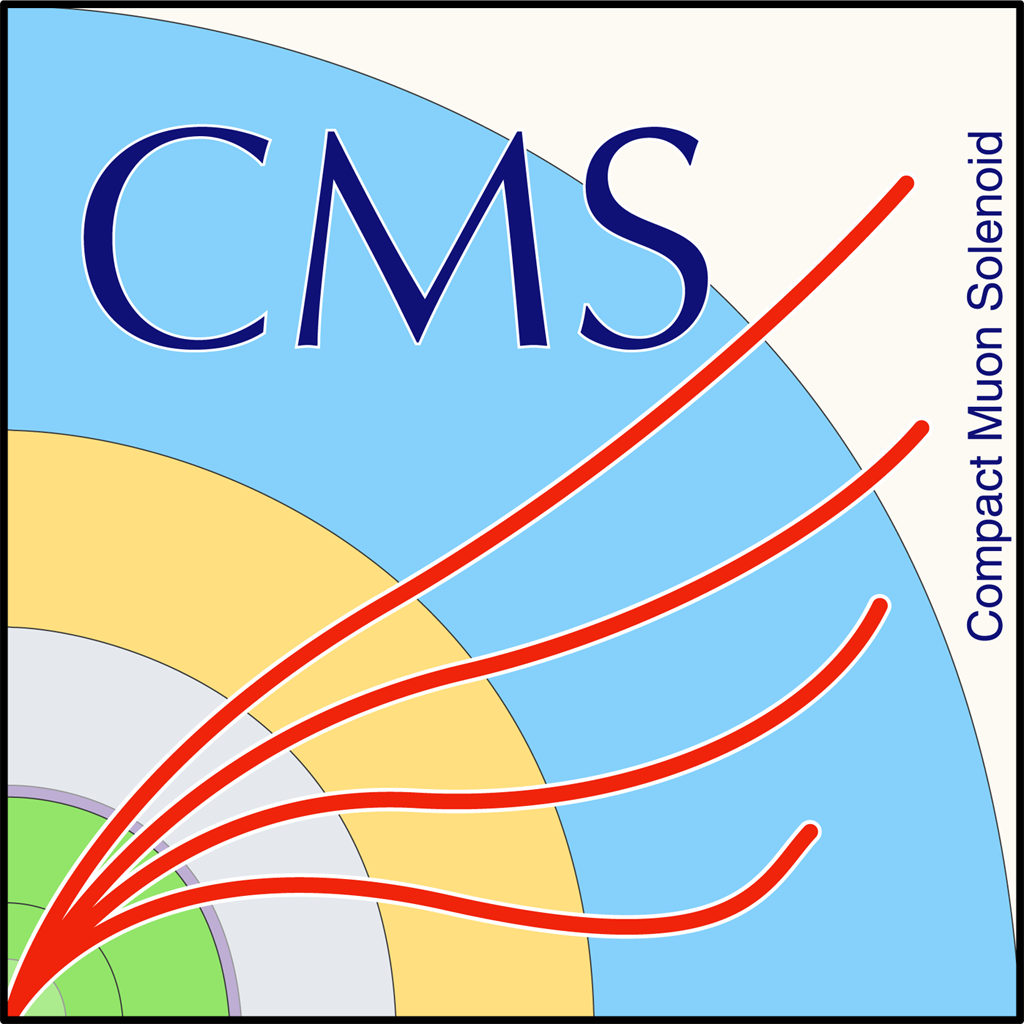
\includegraphics[height=9mm,width=9mm,keepaspectratio]{images/logo_CMS}
\end{textblock*}}


%\usepackage{biblatex}
%\bibliography{bibliography}

%% \setbeamertemplate{footline}[text line]{%
%%   \parbox{\linewidth}{\vspace*{-8pt}some text\hfill\insertshortauthor\hfill\insertpagenumber}}
%% \setbeamertemplate{navigation symbols}{}



\begin{document}

%% Slide 1

\date{ July 10, 2018}
\title[Improving efficiency of analysis jobs in CMS | CHEP2018]{Improving efficiency of analysis jobs in CMS. \\}
\author[Todor Ivanov, University of Sofia ``St. Kliment Ohridski'']{Todor Ivanov on behalf of CRAB Team,\\
CHEP2018}


\begin{frame}{}

\begin{textblock*}{100mm}(\textwidth,-1cm)
    
\includegraphics[height=1cm,width=1cm,keepaspectratio]{images/logo_su}
\end{textblock*}

\begin{textblock*}{100mm}(-8mm,-14mm)
    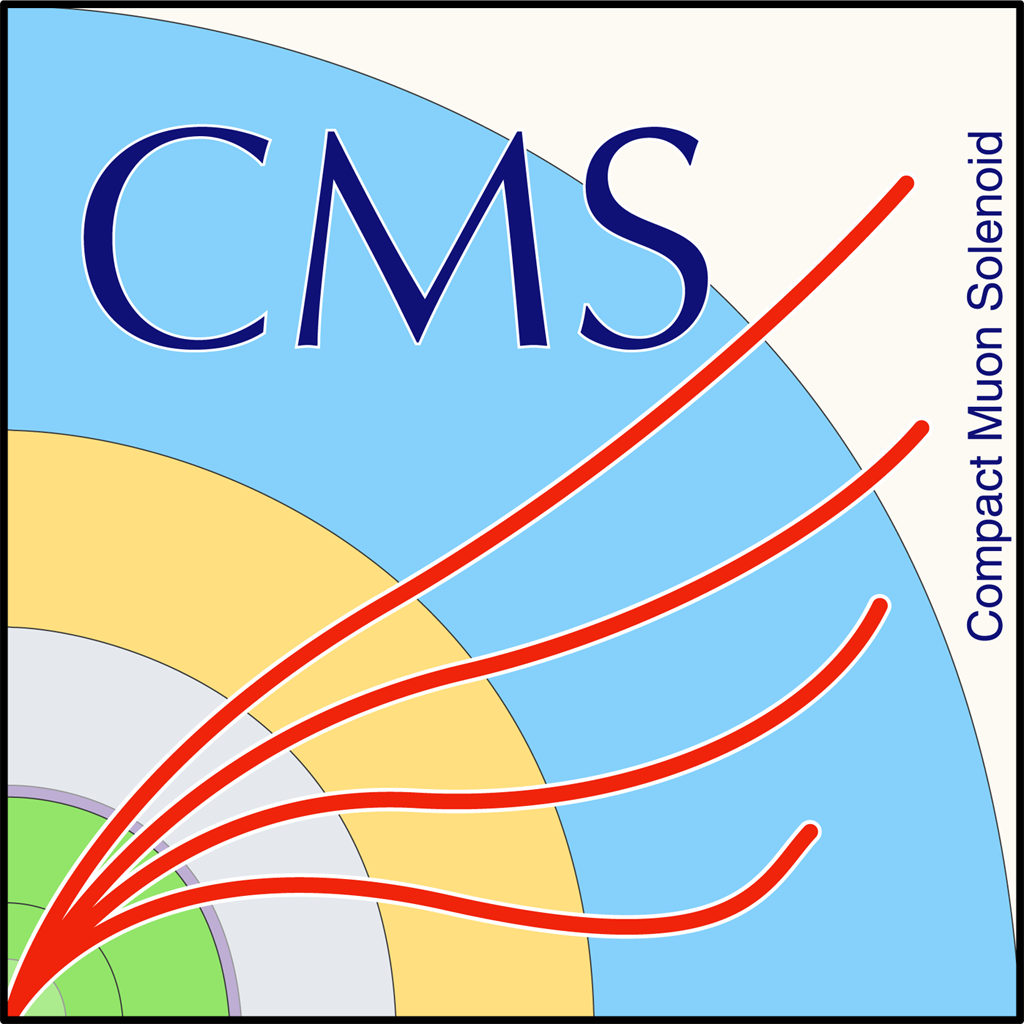
\includegraphics[height=9mm,width=9mm,keepaspectratio]{images/logo_CMS}
\end{textblock*}

  \begin{minipage}[t]{1\textwidth}
    \begin{center}
      \vspace{-1cm}
%      University of Sofia ``St. Kliment Ohridski''\\
%      CRAB Team CMS
    \end{center}
  \end{minipage}
 \noindent\makebox[\linewidth]{\rule{\paperwidth}{1pt}}
 \titlepage

 \vfill

\end{frame}


\section[Problem]{Problem}
\subsection[Problem]{Problem}


\begin{frame}[fragile]{Problem:}

  \begin{itemize}
  \item
    \textbf{The primary need:} to achieve a better resource utilisation
  \item
    \textbf{The secondary need:} to protect the sites from being flooded with jobs they cannot process || serve data for them.
  \item
   \textbf{The old Overflow mechanism} - what does it suffer from:
    \begin{itemize}
    \item
      Statically defined overflow regions -  can't be based on other criteria characterizing ``proximity''
    \item
      Overflow matching decision happens in the timescale of pilot lifetimes -  not flexible enough to respond to faster changes in the status of the distributed CPU and storage resources
    \item
      Requires additional FE groups to be set - a limitation in practice to the different number of settings that could be configured at once.
    \item
      Based on a special type of pilots - fragmentation of the resources, increasing wastage
    \end{itemize}
  \end{itemize}

\end{frame}


\section[Solution]{Solution}
\subsection[Proposed Solution]{Proposed Solution}

\begin{frame}[fragile]{Proposed Solution: }
  A solution based on the condor JobRouter mechanism to edit jobs in place.\\
  \textbf{Challenges:}
  \begin{itemize}
  \item
    The difficulties for the estimation - the complexity in putting the right algorithms:\\
    What do we want to overflow \& Where do we want to send it.\\
    \textit{Sysadmin on a military drill.}
  \item
    The difficulties of measuring:\\
    Hard to find the proper metric which best describes one's needs and the effect of his actions.\\
    \textit{one possibility: IO waits accessible directly from the UserLog @ the Schedd}
  \item
    The complexity of applying all the decisions (separately/together)
  \item
    Decentralizing it adds complexity to the communication between the entities and increases the time for achieving coherency.
  \item
    In the new CMS computing model \textbf{Bandwidth \& IO} should be treated as a separate resource in addition to \textbf{CPU \& Storage}
  \end{itemize}

  %% \begin{itemize}
  %% \item<1-5>
  %%   pass
  %% \item<2-5>
  %%   pass
  %% \item<3-5>
  %%   pass
  %% \end{itemize}
\end{frame}


\subsection[History]{History}
\begin{frame}[fragile]{History - TimeTuner:}
  The first attempt to exploit the CondorJobRouter machinery.\\
  It definitely works fine - it scales and is doing what it is expected to do.\\
  \textbf{What kind of problems did we face:}
  \begin{itemize}
  \item
    Proper communication with the external systems.
  \item
    Time delays in the returned information.
  \item
    Correct monitoring.
  \item
    Efficiency.
  \item
    To protect the JobRouter.
  \item
    To protect the Collector - we basically did not go out of the schedds themselves.
  \end{itemize}
  \textbf{What did we learn:}
  \begin{itemize}
  \item
    One cannot solve a problem which does not exist.
  \item
    One cannot measure the world while looking at his internal load.
  \end{itemize}
  \textbf{We came to the current sate step by step.}
  \begin{itemize}
  \item
    Implementing a maximum overflow in a country and providing a way to substitute the old Overflow.
  \item
    Facing the Tier1 problem - Critical for us. In the current situation of the negotiation order Analysis jobs cannot
    run on the Tier1 sites but there are datasets that are currently placed only at T1.
  \end{itemize}
\end{frame}

\subsection[Current Implementation]{Solution}

\begin{frame}[fragile]{JobAutoTuner and CRAB3 Workflow:}

  \begin{columns}

    \begin{column}[T]{7cm}
      What ever we do we do it at the final step, just before the job submission and after the DAG Expansion - We have to be really fast:
      \begin{itemize}
      \item
        Fast Script execution.
      \item
        Fast in gathering of the Condor related information.
      \item
        Fast in querying the external information.
      \item
        Fast in taking the decisions.
      \item
        Fast in applying it - editing the jobs.
      \end{itemize}
      Alternative solution - keep jobs in hold while measuring (Potential enormous delay in submission time).
    \end{column}

    \begin{column}[T]{5cm}
      {\shadowbox{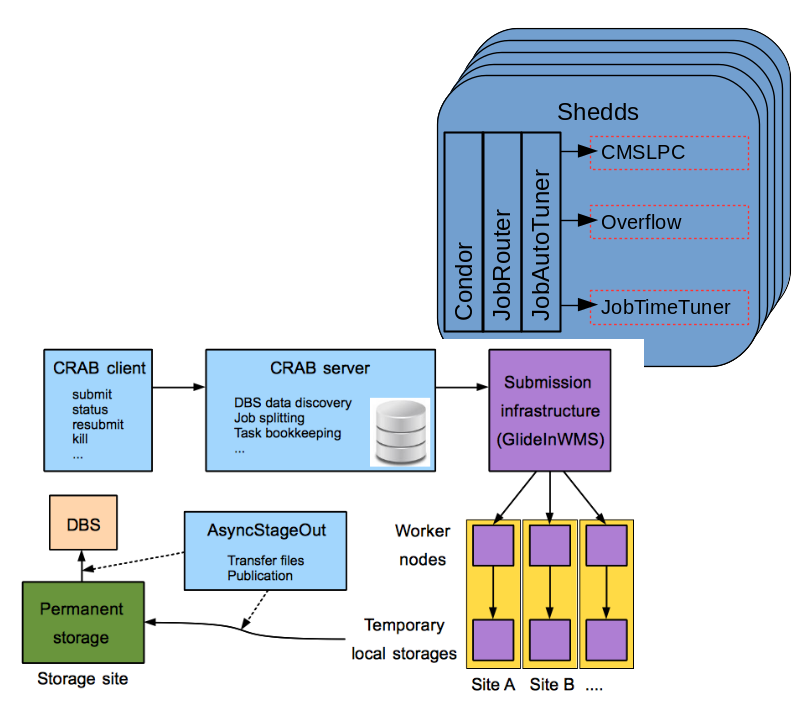
\includegraphics[width=4.5cm]{CRAB3_architecture_simple_JAT}}}
    \end{column}
  \end{columns}

\end{frame}

\begin{frame}[fragile]{Structure:}
  \begin{columns}
    \begin{column}[T]{5cm}
      Three basic abstractions:
      \begin{itemize}
      \item
        \textbf{Information Lifetime:}
        \begin{itemize}
        \item
          static
        \item
          dynamic
        \end{itemize}
      \item
        \textbf{The OverflowLevel:}
        \begin{itemize}
        \item
          PERTASK
        \item
          PERJOB
        \item
          PERBLOCK
        \item
          PERFILE
        \item
          PERDATASET
        \end{itemize}
      \item
        \textbf{The OverflowType:}
        \begin{itemize}
        \item
          GEO
        \item
          TIER1
        \item
          TIER2
        \item
          DATALOCATION
        \item
          LOCALLOAD
        \item
          SRCLOAD
        \item
          DSTLOAD
        \end{itemize}
      \end{itemize}
    \end{column}
    \begin{column}[T]{7cm}
      {\shadowbox{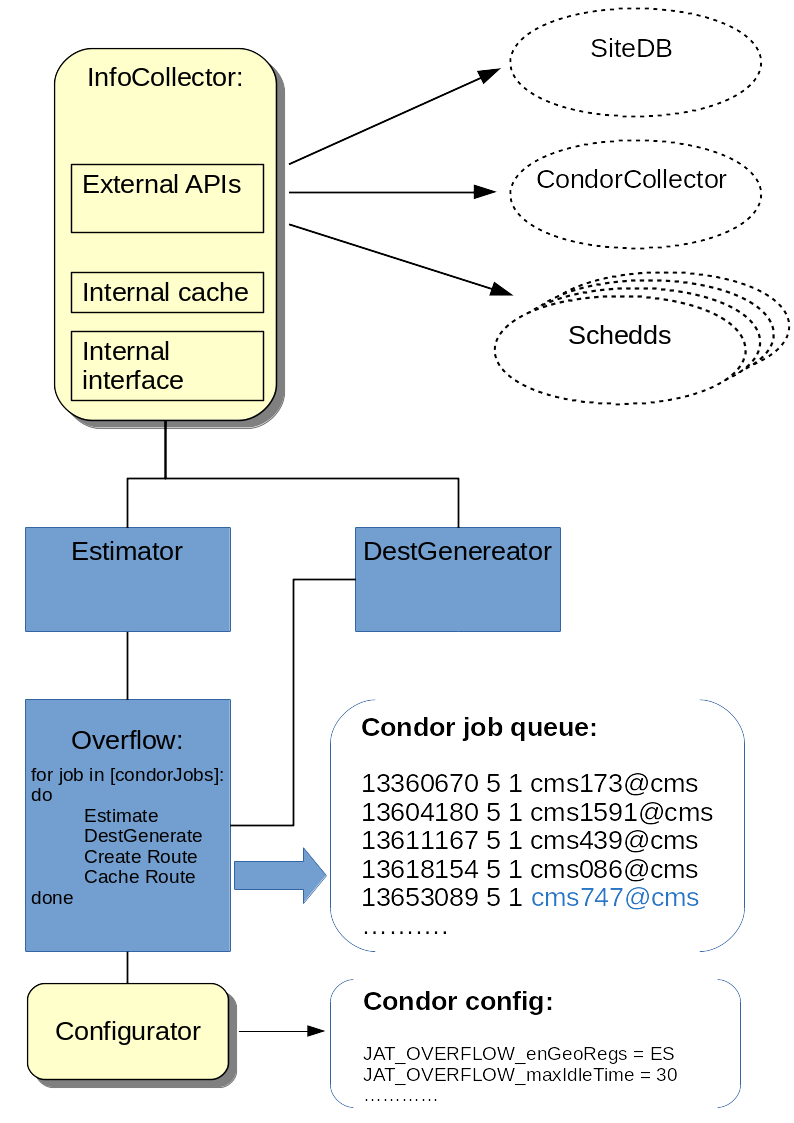
\includegraphics[width=5cm]{CRAB3_overflow}}}
    \end{column}
  \end{columns}
\end{frame}

\begin{frame}[fragile]{Decision making \& Subsets}
  \begin{columns}
    \begin{column}[T]{5cm}
      \begin{itemize}
      \item
        Weighted sum vs. Weighted single decision.
      \item
        Estimating the weights could be dynamic:\\
        In the future we can apply more elaborate mechanisms for estimating the optimal weights according to the prompt feedback about the reaction of the system.
      \item
        Subsets intersections.
      \end{itemize}
    \end{column}
    \begin{column}[T]{7cm}
      {\shadowbox{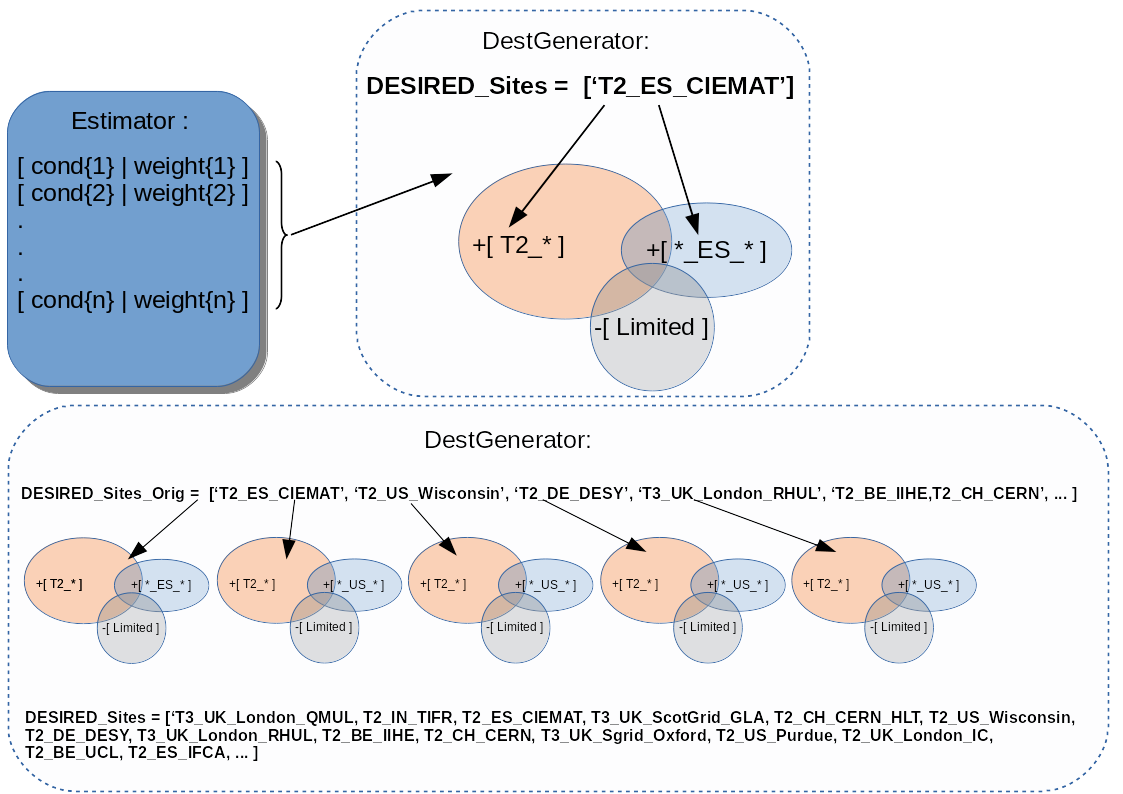
\includegraphics[width=6.5cm]{CRAB3_site_subsets}}}
    \end{column}
  \end{columns}
\end{frame}



\begin{frame}[shrink]{Limits \& Protect ourselves}
  \textbf{Limitations - where and how can be implemented:}\\
  We do not want to shoot ourselves in the thumb - so we need to have more options than just maximum overflow.\\
  \textbf{Alternatives:}\\
  \begin{itemize}
  \item
    \textbf{At the Schedd level} - Inside the script:\\
    Implemented but we cannot say how much can we scale with that.
    \begin{itemize}
    \item
      \textbf{Pros:}\\
      We will have the system solid and configured at one place.\\
      The configuration limits are going to be accessible through the script itself.
    \item
      \textbf{Cons:}\\
      It requires addition queries to the collector (schedds).\\
      Additional delays.\\
      Additional memory for the caching system.\\
    \end{itemize}
  \item
    \textbf{At the Negotiator level} - Concurrency limits.\\
        \begin{itemize}
        \item
          \textbf{Pros:}\\
          Fast solution. Not requiring additional coding.
        \item
          \textbf{Cons:}\\
          We will have the system configured in many places.\\
          Need additional cycle during the negotiation process - creates more pressure on it.\\
          We will brake the possibility to propagate the feedback information (we will not be able to recognise if we hit the limit set in the negotiator or some capacity limit).
        \end{itemize}
  \end{itemize}
\end{frame}



\begin{frame}[fragile]{Current Status:}
  \begin{itemize}
  \item
   \textbf{What is already done:}
    \begin{itemize}
    \item
      \textbf{Information Lifetime:}
      The caching system of the script is working well.\\
    \item
      \textbf{The OverflowLevel:}
      \begin{itemize}
      \item
        PERTASK - implemented \& tested
      \item
        PERJOB - implemented \& under testing
      \item
        PERBLOCK - R\&D
      \item
        PERFILE - R\&D
      \item
        PERDATASET - R\&D
      \end{itemize}
    \item
      \textbf{The OverflowType:}
      \begin{itemize}
      \item
        GEO - implemented \& tested - (Default)
      \item
        TIER1 - implemented \& under testing
      \item
        TIER2 - to be discussed
      \item
        DATALOCATION - R\&D
      \item
        LOCALLOAD - to be discussed
      \item
        SRCLOAD - R\&D
      \item
        DSTLOAD - R\&D
      \end{itemize}
    \end{itemize}
  \item
    \textbf{What is left to be done (near future):}
    \begin{itemize}
    \item
      A proper monitoring and a scale test.
    \item
      Moving it to a daemon.
    \item
      Finalising the rest of the OverflowLevels.
    \item
      Refactoring the Destination Generation in order to better tie it to the way we do the decision making.
    \end{itemize}
  \item
    \textbf{What can be done in the future:}
    \begin{itemize}
    \item
      To make it possible to measure the actual situation (load / resource utilisation) at the sites  and mechanism for propagating the feedback.
    \item
      To have more topology aware information accessible.
    \item
      A hard one: to make it more general and context independent.
    \end{itemize}
  \end{itemize}

\end{frame}


%% \begin{frame}[fragile]{Quantitative Results}
%%   pass
%% \end{frame}

%% \begin{frame}[fragile]{What is left to be done}
%%   pass
%% \end{frame}

\end{document}






